\section{Descrição}
A aplicação usa a linguagem \textit{Python} com o framework \textit{CherryPy} para expô-la como um serviço com interface web e o módulo \textit{boto} para acessar o Amazon SimpleDB.
Ela apresenta uma tela onde o usuário entra com seu nome, caso já não tenha iniciado uma sessão(figura 3.4), e outra onde ele  pode visualizar e criar tarefas, além de marcá-las como "concluídas"(figura 3.5).

\subsection{Organização dos dados}
A aplicação utiliza apenas um domínio, chamado \textbf{TaskManagerDomain}. Nesse domínio, cada item consiste em uma tarefa, sendo o nome do item a palavra 'Task' seguida de um identificador numérico que é autoincrementado a cada nova tarefa criada. No mesmo domínio, há um item chamado \textit{maxId}, cujo único atributo se chama \textit{value} e armazena o maior identificador presente no domínio. A cada nova tarefa, esse valor é incrementado.\\
Cada tarefa possui os atributos \textit{text}(a descrição da tarefa), \textit{author}(nome do autor da tarefa), \textit{done}(booleano indicando se a tarefa está concluída) e \textit{created{\textunderscore}at}(data de criação da tarefa). A representação dos dados pode ser vista na figura 3.6.

\subsection{Organização do código}
O código possui duas classes:
\begin{itemize}
	\item \textbf{SdbBridge}: responsável por prover uma interface de acesso simplificada para criar, alterar e recuperar tarefas do banco de dados;
	\item \textbf{Task}: essa classe expõe métodos para manipulação e visualização de tarefas com uma interface REST através do framework \textit{CherryPy}.
\end{itemize}

\begin{figure}
	\centering
	\fbox{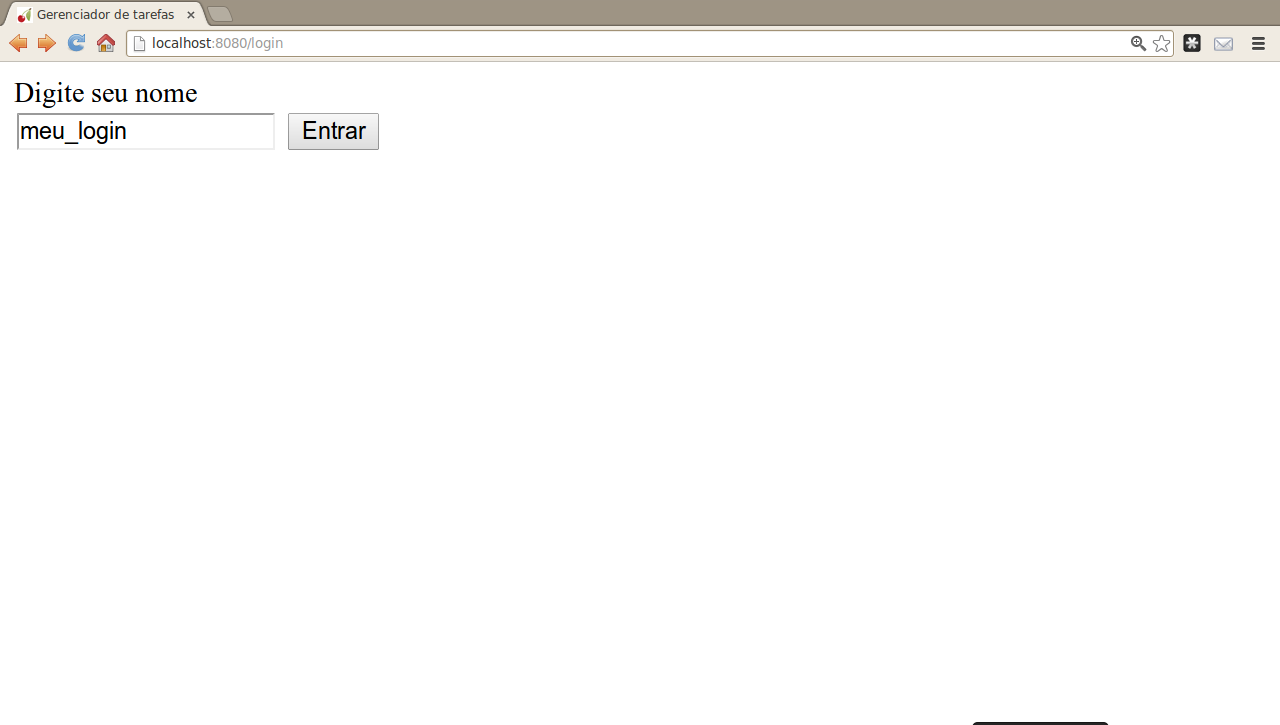
\includegraphics[scale=0.3]{figuras/task_manager_login_screen.png}}
	\label{fig:app_tela_login}
	\caption{Tela de login}
\end{figure}

\begin{figure}
	\centering
	\fbox{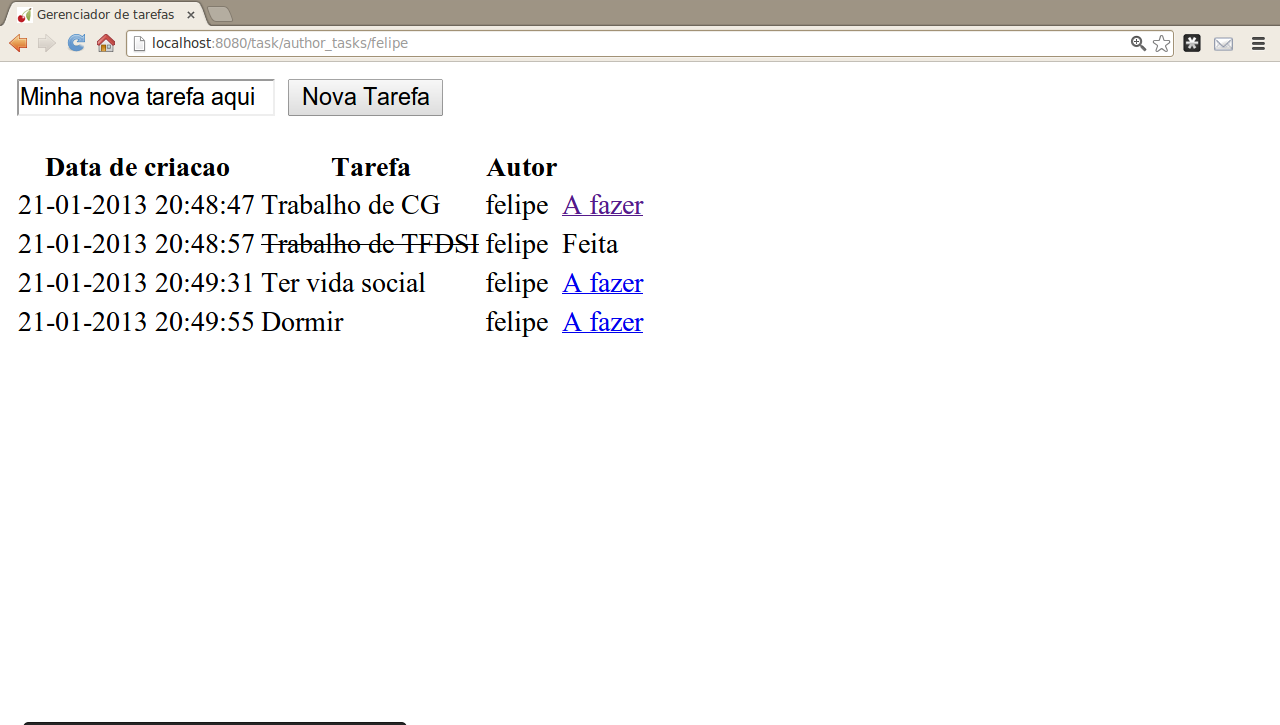
\includegraphics[scale=0.3]{figuras/task_manager_tasks_screen.png}}
	\label{fig:app_tela_tarefas}
	\caption{Tela de gerenciamento de tarefas}
\end{figure}

\begin{figure}
	\centering
	\fbox{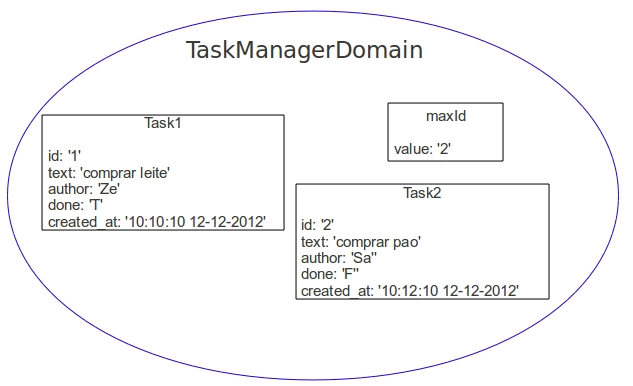
\includegraphics[scale=0.6]{figuras/taskdomain.jpg}}
	\label{fig:task_domain}
	\caption{Dados utilizados na aplicação de exemplo}
\end{figure}